\documentclass[mathserif, handout]{beamer}

\usepackage{url}
% ======================================================================
% General LaTeX Setup for Beamer (Reusable Preamble)
% Author: Chandra Gummaluru
% ======================================================================

\documentclass[mathserif, handout]{beamer}
\setbeamertemplate{frametitle}{}

% ------------------------------------------------------------
% basic packages
% ------------------------------------------------------------
\usepackage{url}
\usepackage{ifthen}
\usepackage{enumerate}
\usepackage[font=small]{caption}
\usepackage{subcaption}
\usepackage{moresize}
\usepackage[outline]{contour}
\usepackage{transparent}
\usepackage{worldflags}
\usepackage{bm}
\usepackage{graphbox}
\usepackage{mathtools}
\usepackage{multirow}
\usepackage{fontawesome5}
\usepackage{pifont}
\usepackage{array}
\usepackage{comment}

% ------------------------------------------------------------
% math
% ------------------------------------------------------------
\DeclarePairedDelimiter{\floor}{\lfloor}{\rfloor}
\DeclarePairedDelimiter{\ceil}{\lceil}{\rceil}

% ------------------------------------------------------------
% colors
% ------------------------------------------------------------
\definecolor{hl}{RGB}{248,196,69}
\definecolor{myred}{HTML}{ED5565}
\definecolor{myorange}{HTML}{FC6E51}
\definecolor{myyellow}{HTML}{FFCE54}
\definecolor{mycyan}{HTML}{4FC1E9}
\definecolor{myblue}{HTML}{5D9CEC}

\newcommand{\graytext}[1]{\footnotesize\color{gray}#1\normalsize\color{black}}

% ------------------------------------------------------------
% symbols
% ------------------------------------------------------------
\newcommand{\cmark}{\ding{51}}
\newcommand{\xmark}{\ding{55}}

% ------------------------------------------------------------
% highlighting
% ------------------------------------------------------------
\newcommand{\reducedstrut}{\vrule width 0pt height .9\ht\strutbox depth .9\dp\strutbox\relax}
\newcommand{\highlight}[1]{%
  \begingroup\setlength{\fboxsep}{0pt}\colorbox{hl}{\reducedstrut$\displaystyle #1$\/}\endgroup}
\newcommand{\highlightc}[2]{%
  \begingroup\setlength{\fboxsep}{0pt}\colorbox{#1}{\reducedstrut$\displaystyle #2$\/}\endgroup}

% ------------------------------------------------------------
% environments (boxes)
% ------------------------------------------------------------
\usepackage{tcolorbox}
\tcbuselibrary{skins}

\newtcolorbox{thmbox}[1][]{colback=gray!30!white!20, colframe=black, fonttitle=\bfseries, title=#1, boxrule=0.5pt}

% 1) Bottom open (draw top + sides only)
\newtcolorbox{thmboxtop}[1][]{
    enhanced,
    frame hidden,
    colback=gray!30!white!20,
    borderline north={0.5pt}{0pt}{black}, % top
    borderline west={0.5pt}{0pt}{black},  % left
    borderline east={0.5pt}{0pt}{black}   % right
}

% 2) Top open (draw bottom + sides only)
\newtcolorbox{thmboxbot}[1][]{
    enhanced,
    frame hidden,
    colback=gray!30!white!20,
    borderline south={0.5pt}{0pt}{black}, % bottom
    borderline west={0.5pt}{0pt}{black},  % left
    borderline east={0.5pt}{0pt}{black}   % right
}

% 3) Side only (draw only left and right)
\newtcolorbox{thmboxside}[1][]{
    enhanced,
    frame hidden,
    colback=gray!30!white!20,
    borderline west={0.5pt}{0pt}{black},  % left
    borderline east={0.5pt}{0pt}{black}   % right
}

\newtcolorbox{defboxtop}[1][]{
    enhanced,
    colback=gray!30!white!20,
    frame hidden,
    overlay={
        % Draw top + sides with rounded corners
        \draw[line width=0.5pt, black, rounded corners=3mm]
            (frame.south west) -- (frame.north west) -- (frame.north east) -- (frame.south east);
    },
    #1
}

\newtcolorbox{defboxbot}[1][]{
    enhanced,
    colback=gray!30!white!20,
    frame hidden,
    overlay={
        % Draw top + sides with rounded corners
        \draw[line width=0.5pt, black, rounded corners=3mm]
            (frame.north west) -- (frame.south west) -- (frame.south east) -- (frame.north east);
    },
    #1
}

\newtcolorbox{defboxside}[1][]{
    enhanced,
    frame hidden,
    colback=gray!30!white!20,
    borderline west={0.5pt}{0pt}{black},  % left
    borderline east={0.5pt}{0pt}{black}   % right
}

\newtcolorbox{proofbox}[1][]{colback=gray!20!white!20, colframe=grey, fonttitle=\bfseries, title=#1, boxrule=0.5pt, colbacktitle=white, enhanced jigsaw, sharp corners}

% ------------------------------------------------------------
% code listings
% ------------------------------------------------------------
\usepackage{listings}
\lstdefinestyle{mypython}{
  language=Python,
  deletekeywords=[2]{open, next, from, chr, str, int},
  morekeywords=[3]{List, Graph, Tree, Dict, Set, UnionFind, Ordict, Trie, Queue},
  morekeywords=[4]{ListNode, Vertex, Edge, Path, TreeNode, DictNode, UnifNode, OrdictNode, TrieNode, QueueNode},
  morekeywords=[5]{True, False, Boolean, String, Integer, Key, Function, KeyedObject, Object, Array, Tuple, Optional, None},
  keywordstyle=\color{mycyan}\bfseries,
  keywordstyle=[3]\color{myblue}\bfseries,
keywordstyle=[4]\color{myblue}\bfseries,
keywordstyle=[5]\color{mycyan}\bfseries,
  stringstyle=\color{orange},
  commentstyle=\color{gray}\itshape,
  basicstyle=\ttfamily\footnotesize,
  numbers=left,
  numberstyle=\tiny\color{gray},
  stepnumber=1,
  numbersep=5pt,
  xleftmargin=15pt,
  frame=none,
  showstringspaces=false,
  breaklines=true,
  breakatwhitespace=true,
  tabsize=4,
  columns=flexible
}


% ------------------------------------------------------------
% algorithms
% ------------------------------------------------------------
\usepackage{algorithm}
\usepackage[endLComment=~]{algpseudocodex}
\makeatletter
\algrenewcommand\ALG@beginalgorithmic{\footnotesize}
\makeatother

% ------------------------------------------------------------
% optimization environments
% ------------------------------------------------------------
\usepackage[nocomma]{optidef}

% ------------------------------------------------------------
% pgfplots and pie charts
% ------------------------------------------------------------
\usepackage{pgfplots}
\usepackage{pgf-pie}
\pgfplotsset{compat=1.7}

% ------------------------------------------------------------
% tikz
% ------------------------------------------------------------
\usepackage{tikz}
\usetikzlibrary{
  angles, quotes, positioning, fit, backgrounds, shapes.geometric, intersections,
  calc, shapes, mindmap, decorations.text, arrows, arrows.meta,
  automata, chains, decorations.pathreplacing, calligraphy,
  decorations.markings, shapes.misc, decorations.pathmorphing
}
\tikzset{
  invisible/.style={opacity=0},
  visible on/.style={alt=#1{}{invisible}},
  alt/.code args={<#1>#2#3}{\alt<#1>{\pgfprioritysalso{#2}}{\pgfprioritysalso{#3}}}
}

\newcommand{\multiedge}[5][]{
\pgfmathsetmacro{\N}{#4}
\pgfmathsetmacro{\mid}{(\N-1)/2}
\foreach \i in {0,...,\numexpr#4-1\relax} {

\pgfmathsetmacro{\k}{\i-\mid}
\draw[#1] ($ (#2) + \k*#5*($(#2)!1!90:(#3)$) $) -- ($ (#3) + \k*#5*($(#2)!1!90:(#3)$) $); 

}
\draw[#1,  -{>[scale=1]}]
  ($(#2)!0.54!(#3)$) -- ($(#2)!0.55!(#3)$);
}

% ------------------------------------------------------------
% bibliography
% ------------------------------------------------------------
\usepackage[style=ieee]{biblatex}
\setbeamertemplate{bibliography item}{\insertbiblabel}
\setbeamertemplate{background canvas}{
  \begin{tikzpicture}[remember picture,overlay]
    \node[opacity=0.0075]
      at (current page.center)
      {
\includegraphics[width=0.8\paperwidth]{images/signature.pdf}};
  \end{tikzpicture}
}

% ------------------------------------------------------------
% beamer theme and settings
% ------------------------------------------------------------
\usetheme{Boadilla}
\usecolortheme{seagull}
\beamertemplatenavigationsymbolsempty
\setbeamertemplate{enumerate item}{(\arabic{enumi})}
\setbeamertemplate{enumerate subitem}{(\alph{enumii})}
\setbeamertemplate{enumerate subsubitem}{(\roman{enumiii})}
\setbeamertemplate{itemize item}[circle]
\setbeamertemplate{itemize subitem}{\circ}
\setbeamertemplate{itemize subsubitem}{-}
\setbeamercolor{item}{fg=black!40}
\setbeamercovered{transparent=10}

% ===========================
% Premade TikZ Figure Commands
% ===========================

% images w/ labels
% inside tikz as a node
\NewDocumentCommand{\labeledimgnodetikz}{O{} m m m m m m}{%
	\begin{scope}[transparency group, #1]
		\node[
			draw,
			circle,
			inner sep=0,
			outer sep=0,
			minimum size=10mm,
			#1
		] (#5) at (#3,#4)
		{\includegraphics[scale=#7]{#6}};
		\node[
			rectangle,
			draw=black,
			thick,
			fill=black!55,
			rounded corners=0.1mm,
			inner sep=0pt,
			outer sep=0pt,
			minimum size=2.8mm,
			minimum width=3.5mm
		] at (#3,#4-0.1) {};
		\node[outer sep=0, inner sep=0, white] at (#3,#4-0.1) {\footnotesize #2};
	\end{scope}
}

% inside tikz isolated

% outside tikz
\NewDocumentCommand{\labelednode}{m}{%
	\begin{tikzpicture}[baseline={(0,-1mm)}]
		\node[
			rectangle,
			thick,
			draw=black,
			fill=black!55,
			rounded corners=0.1mm,
			inner sep=0pt,
			outer sep=0pt,
			minimum size=2.8mm,
			minimum width=3.5mm
		] at (0,0) {};
		\node[outer sep=0, inner sep=0, white, minimum size=2.8mm, minimum width=3.5mm] at (0,0) {\footnotesize #1};
	\end{tikzpicture}
}

% images only
% inside tikz as a node
\NewDocumentCommand{\imgnodetikz}{O{} m m m m m m}{%
	\begin{scope}[transparency group, #1]
		\node[
			draw,
			circle,
			inner sep=0,
			outer sep=0,
			minimum size=10mm,
			#1
		] (#5) at (#3,#4)
		{\includegraphics[scale=#7]{#6}};
		\node[
			rectangle,
			draw,
			thick,
			fill=black!55,
			rounded corners=0.1mm,
			inner sep=0pt,
			outer sep=0pt,
			minimum size=2.8mm,
			minimum width=3.5mm,
			opacity=0
		] at (0,0) {};
		\node[outer sep=0, inner sep=0, white, opacity=0] at (0,0) {\footnotesize #2};
	\end{scope}
}

% inside tikz isolated
\NewDocumentCommand{\imgtikz}{O{} mm}{%
	\begin{scope}[transparency group, #1]
		\node[
			inner sep=0,
			outer sep=0
		] (#5) at (#3,#4)
		{\includegraphics[scale=#3]{#2}};
	\end{scope}
}


% outside tikz
\NewDocumentCommand{\imgnode}{mm}{%
	\begin{tikzpicture}[baseline={(0,-1mm)}]
        \node[
            inner sep=0,
            outer sep=0,
            draw opacity=0,
        ] at (0,0)
        {\includegraphics[scale=#2]{#1}};
    \end{tikzpicture}
}

% outside tikz (inline)
\newcommand{\imgnodetext}[2]{%
	\hspace{-0.5mm}%
	\raisebox{-0.26\height}{%
		\includegraphics[scale=#2]{#1}%
	}%
	\hspace{-0.5mm}%
}


% labels only
% inside tikz as a node
\NewDocumentCommand{\labeltikz}{m}{%
	\node[
		rectangle,
		thick,
		draw=black,
		fill=black!55,
		rounded corners=0.1mm,
		inner sep=0pt,
		outer sep=0pt,
		minimum size=2.8mm,
		minimum width=3.5mm
	] at (0,0) {};
	\node[outer sep=0, inner sep=0, white, draw opacity=0] at (0,0) {\footnotesize #1};
}

% inside tikz isolated

% outside tikz

% === define custom pgfkeys ===
\pgfkeys{
	/devicenode/.is family, /devicenode,
	outline thickness/.initial=thick,
	outline color/.initial=black
}

\NewDocumentCommand{\qpacket}{m}{%
	\begin{tikzpicture}[baseline=(current bounding box.center)]
		\node at (0.5,0.4) {\includegraphics[scale=0.1]{#1}};
	\end{tikzpicture}%
}

\NewDocumentCommand{\bpacketid}{mmm}{%
	\begin{tikzpicture}[baseline=(current bounding box.center)]
		\begin{scope}[shift={(0.85,0.7)}]
			\draw[thick, draw=black, fill=#1, rounded corners=1pt] (0.01,0.05) rectangle node[white, text width=1cm, align=center] {\color{#3}\footnotesize #2} (-0.71,-0.625);
		\end{scope}
	\end{tikzpicture}%
}

\NewDocumentCommand{\packetid}{mmmm}{%
	\begin{tikzpicture}[baseline=(current bounding box.center)]
		\begin{scope}[shift={(0.85,0.7)}]
			\draw[thick, draw=black, fill=#2, rounded corners=1pt] (0.01,0.05) rectangle node[white, text width=1cm, align=center] {\color{#4}\footnotesize #3} (-0.71,-0.625);
			\node[
				star,
				star points=30,
				star point ratio=0,
				scale=1.5,
				draw=black,
				thick,
				fill=white,
				rounded corners=0.1mm,
				inner sep=0pt,
				minimum size=2.8mm
			] at (0,0) {};
			\node at (0,0) {\footnotesize #1};
		\end{scope}
	\end{tikzpicture}%
}

\tikzset{
	dictnode/.pic={
			\draw[thick, fill=#1, line join=]
			(-0.75,-0.5) --
			(-0.75,0.5)  --
			(0.75,0.5) --
			(0.75,-0.5) --
			cycle --
			(-0.75, 0.75) --
			(0.75, 0.75) --
			(0.75, -0.5) --
			cycle;
		}
}

\tikzset{
	queuenode/.pic={
			\draw[thick, fill=#1, line join=round]
			(-0.85,-0.5) --
			(-0.85,0.5)  --
			(0.65,0.5) --
			(0.75,0) --
			(0.65,-0.5) --
			cycle;
		}
}

\tikzset{
	queuenodetail/.pic={
			\draw[thick, fill=#1, line join=round]
			(-0.75,-0.5) --
			(-0.75,0.5)  --
			(0.65,0.5) --
			(0.75,0) --
			(0.65,-0.5) --
			cycle;
		}
}

\tikzset{
	listnode/.style={
			shape=rectangle,
			rounded corners,
			thick,
			minimum height=10mm,
			minimum width=15mm,
			inner sep=0pt
		}
}

\tikzset{
	arraynode/.style={
			shape=rectangle,
			thick,
			minimum height=10mm,
			minimum width=15mm,
			inner sep=0pt
		}
}

\tikzset{
	graphnode/.style={
			shape=circle,
			thick,
			minimum size=5mm,
			inner sep=0pt
		}
}

\tikzset{
	defaultnode/.style={
			transform shape,
			circle,
			draw=black,
			thick,
			fill=white,
			minimum size=10mm,
			inner sep=0pt
		},
	newnode/.style={
			transform shape,
			defaultnode,
			draw=myyellow,
			fill=myyellow!60,
			very thick
		},
	newnodelight/.style={
			transform shape,
			defaultnode,
			draw=myyellow,
			fill=myyellow!30,
			very thick
		},
	deletenode/.style={
			defaultnode,
			draw=gray,
			dashed,
			fill=lightgray,
			text=gray,
			very thick
		},
	nooutlinenode/.style={
			defaultnode,
			draw=none,
            draw opacity=0,
			text=black,
			very thick
		},
    nofillnode/.style={
			defaultnode,
			fill=none,
            text=black,
			very thick
		}
}
\tikzset{
	faded/.style={opacity=0.5, text opacity=0.5, transparency group}
}
\tikzset{
	smallgraytext/.style={font=\footnotesize\color{gray}}
}
\tikzset{
	graytext/.style={font=\normalsize\color{gray}}
}
\tikzset{
  squigglearrow/.style={
    very thick,
    lightgray,
    decorate,
    decoration={
      snake,
      amplitude=1.75pt,
      segment length=8pt
    }
  }
}



\usetikzlibrary{shapes.gates.logic.US}

\newcommand{\ttab}[1]{\texttt{#1}}

% ------------------------------------------------------------
% simplified MOSFET symbols (course style: gate on the left,
% source on top, drain on the bottom; a bubble marks pMOS)
% terminals when placed at (x,y):
%   gate   = (x,y)+(-0.6,0)
%   source = (x,y)+(0,0.6)
%   drain  = (x,y)+(0,-0.6)
% ------------------------------------------------------------
\tikzset{
  nmos/.pic={
    \draw[thick] (0,0.6) -- (0,0.22);
    \draw[thick] (0,-0.6) -- (0,-0.22);
    \draw[thick] (0,-0.22) -- (0,0.22);
    \draw[thick] (-0.28,0.26) -- (-0.28,-0.26);
    \draw[thick] (-0.6,0) -- (-0.28,0);
  },
  pmos/.pic={
    \draw[thick] (0,0.6) -- (0,0.22);
    \draw[thick] (0,-0.6) -- (0,-0.22);
    \draw[thick] (0,-0.22) -- (0,0.22);
    \draw[thick] (-0.32,0.26) -- (-0.32,-0.26);
    \draw[thick] (-0.6,0) -- (-0.46,0);
    \draw[thick] (-0.39,0) circle (0.07);
  }
}

% title
\title{Transistors and Logic Gates}
\subtitle{Computer Organization}
\author[C. Gummaluru]{Chandra Gummaluru}
\titlegraphic{
\includegraphics[width=0.15\linewidth]{images/signature.pdf}}
\institute[]{\url{chandra-gummaluru.github.io} }
\date[Computer Organization]{}

\begin{document}

\begin{frame}
  \maketitle
\end{frame}

\begin{frame}
  Recall that we break up the voltage range into two levels.
  \begin{figure}
    \centering
    \begin{tikzpicture}[>=stealth]
      % a wire with a high and low voltage state
      \draw[thick] (0,0) -- (1,0) -- (1,1.2) -- (2,1.2) -- (2,0) -- (3,0);
      \node[smallgraytext, below=7mm of {(1.5,0)}] {voltage over time};

      \node[smallgraytext] at (0.5,-0.5) {low};
      \node[smallgraytext] at (1.5,1.7) {high};
      \node[smallgraytext] at (2.5,-0.5) {low};

      \draw[->, gray, thick] (3.6,0.6) -- (5,0.6);

      \node at (6.3,0.6) {\Large $0 \; \; 1 \;\; 0$};
    \end{tikzpicture}
  \end{figure}
  \begin{center}
  \graytext{a voltage above some upper threshold is read as a \texttt{1}, and a voltage below a lower threshold is read as a \texttt{0}}    
  \end{center}
  
\end{frame}

\begin{frame}
  
  A wire can carry one of thse two values, depending on what it is tied to. \\[7mm]
  \begin{minipage}[t]{0.33\textwidth}
    \centering
    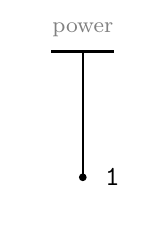
\begin{tikzpicture}[line width=0.9pt, baseline=(current bounding box.north)]
      \useasboundingbox (-0.7,1.2) rectangle (0.7,-1.1);
      % power rail
      \draw[very thick] (-0.4,0.9) -- (0.4,0.9);
      \node[smallgraytext, above=0mm] at (0,0.95) {power};
      \draw (0,0.9) -- (0,-0.7);
      \fill (0,-0.7) circle (1.4pt);
      \node[right=1.5mm] at (0,-0.7) {\ttab{1}};
    \end{tikzpicture} \\[6mm]
    \graytext{connected to power} \\
    \graytext{carries a \texttt{1}}
  \end{minipage}%
  \begin{minipage}[t]{0.33\textwidth}
    \centering
    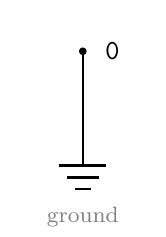
\begin{tikzpicture}[line width=0.9pt, baseline=(current bounding box.north)]
      \useasboundingbox (-0.7,1.2) rectangle (0.7,-1.1);
      \draw (0,0.9) -- (0,-0.55);
      \fill (0,0.9) circle (1.4pt);
      \node[right=1.5mm] at (0,0.9) {\ttab{0}};
      % ground symbol
      \draw (-0.3,-0.55) -- (0.3,-0.55);
      \draw (-0.2,-0.7) -- (0.2,-0.7);
      \draw (-0.1,-0.85) -- (0.1,-0.85);
      \node[smallgraytext, below=0mm] at (0,-0.95) {ground};
    \end{tikzpicture} \\[6mm]
    \graytext{connected to ground}\\
    \graytext{carries a \texttt{0}}
  \end{minipage}%
  \begin{minipage}[t]{0.33\textwidth}
    \centering
    \begin{tikzpicture}[line width=0.9pt, baseline=(current bounding box.north)]
      \useasboundingbox (-0.7,1.2) rectangle (0.7,-1.1);
      % open (unconnected) end
      \draw (0,0.75) circle (0.07);
      \draw (0,0.68) -- (0,-0.7);
      \fill (0,-0.7) circle (1.4pt);
      \node[right=1.5mm] at (0,-0.7) {\ttab{z}};
    \end{tikzpicture} \\[6mm]
    \graytext{connected to nothing}\\
    \graytext{carries an undefined value, \texttt{z}}
  \end{minipage}
\\[7mm]
However, its value can also be undefined if it is not tied to anything (this is different from carrying a \texttt{0}).
\end{frame}

\begin{frame}
Switches allow us to change what a wire is tied to.\\[3mm]
  \begin{minipage}{0.5\textwidth}
    \centering
    \highlight{\textbf{open}} \\[4mm]
    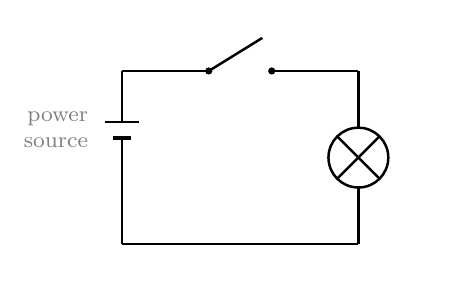
\begin{tikzpicture}[line width=0.9pt]
      \useasboundingbox (-1.2,-0.3) rectangle (3.8,2.75);
      % loop wires
      \draw (0,0) -- (3,0);        % bottom
      \draw (0,0) -- (0,1.35);     % lower left
      \draw (0,1.55) -- (0,2.2);   % upper left
      % battery (power source)
      \draw (-0.22,1.55) -- (0.22,1.55);
      \draw[line width=1.7pt] (-0.11,1.35) -- (0.11,1.35);
      \node[smallgraytext, left=1mm, align=right] at (-0.2,1.45) {power\\source};
      % top wire and switch
      \draw (0,2.2) -- (1.1,2.2);
      \fill (1.1,2.2) circle (1.3pt);
      \fill (1.9,2.2) circle (1.3pt);
      \draw (1.1,2.2) -- (1.78,2.62);   % lever up (open)
      \draw (1.9,2.2) -- (3,2.2);
      % right wire to bulb
      \draw (3,2.2) -- (3,1.48);
      \draw (3,0.72) -- (3,0);
      % bulb (off)
      \draw (3,1.1) circle (0.38);
      \draw (2.73,0.83) -- (3.27,1.37);
      \draw (2.73,1.37) -- (3.27,0.83);
    \end{tikzpicture} \\[4mm]
    \graytext{the switch breaks the loop, \\ so the bulb stays off}
  \end{minipage}%
  \begin{minipage}{0.5\textwidth}
    \centering
    \highlight{\textbf{closed}} \\[4mm]
    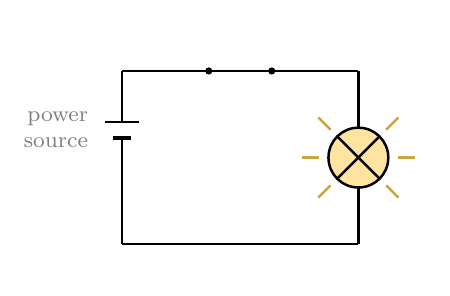
\begin{tikzpicture}[line width=0.9pt]
      \useasboundingbox (-1.2,-0.3) rectangle (3.8,2.75);
      % loop wires
      \draw (0,0) -- (3,0);
      \draw (0,0) -- (0,1.35);
      \draw (0,1.55) -- (0,2.2);
      % battery (power source)
      \draw (-0.22,1.55) -- (0.22,1.55);
      \draw[line width=1.7pt] (-0.11,1.35) -- (0.11,1.35);
      \node[smallgraytext, left=1mm, align=right] at (-0.2,1.45) {power\\source};
      % top wire and switch
      \draw (0,2.2) -- (1.1,2.2);
      \fill (1.1,2.2) circle (1.3pt);
      \fill (1.9,2.2) circle (1.3pt);
      \draw (1.1,2.2) -- (1.9,2.2);     % lever down (closed)
      \draw (1.9,2.2) -- (3,2.2);
      % right wire to bulb
      \draw (3,2.2) -- (3,1.48);
      \draw (3,0.72) -- (3,0);
      % bulb (on)
      \fill[myyellow!55] (3,1.1) circle (0.38);
      \draw (3,1.1) circle (0.38);
      \draw (2.73,0.83) -- (3.27,1.37);
      \draw (2.73,1.37) -- (3.27,0.83);
      \foreach \a in {0,45,135,180,225,315} {
        \draw[myyellow!80!black] ($(3,1.1)+(\a:0.5)$) -- ($(3,1.1)+(\a:0.72)$);
      }
    \end{tikzpicture} \\[4mm]
    \graytext{the switch completes the loop, \\ so the bulb turns on}
  \end{minipage}
  \\[4mm]
  To build a computer, we need to creating a switch that can be moved by sending an electrical signal.
\end{frame}

% ------------------------------------------------------------
% the transistor
% ------------------------------------------------------------
\begin{frame}{The Transistor}
  \begin{center}
    \Large \highlight{\textbf{the transistor}}
  \end{center}
\end{frame}

\begin{frame}
  A transistor has three terminals. The voltage on the \highlight{\textbf{gate}} decides whether current may flow between the \highlight{\textbf{source}} and the \highlight{\textbf{drain}}.
  \begin{figure}
    \centering
    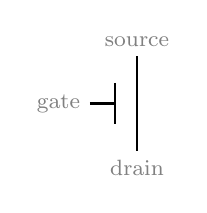
\begin{tikzpicture}
      \pic at (0,0) {nmos};
      \node[smallgraytext, above=0mm] at (0,0.6) {source};
      \node[smallgraytext, below=0mm] at (0,-0.6) {drain};
      \node[smallgraytext, left=0mm] at (-0.6,0) {gate};
    \end{tikzpicture}
  \end{figure}
  \begin{center}
    \graytext{the gate acts like the handle of a switch}
  \end{center}
\end{frame}

\begin{frame}
  Two kinds of transistor respond to the gate in opposite ways.\\[4mm]
  \begin{minipage}{0.5\textwidth}
    \centering
    \highlight{\textbf{nMOS}} \\[3mm]
    \begin{tikzpicture}
      \pic at (0,0) {nmos};
      \draw[thick] (0,0.6) -- ++(0,0.15);
      \draw[thick] (0,-0.6) -- ++(0,-0.15);
      \draw[thick] (-0.6,0) -- ++(-0.15,0) node[left, smallgraytext] {\ttab{g}};
    \end{tikzpicture} \\[3mm]
    \graytext{conducts when the gate \\ is \ttab{1}}
  \end{minipage}%
  \begin{minipage}{0.5\textwidth}
    \centering
    \highlight{\textbf{pMOS}} \\[3mm]
    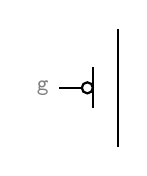
\begin{tikzpicture}
      \pic at (0,0) {pmos};
      \draw[thick] (0,0.6) -- ++(0,0.15);
      \draw[thick] (0,-0.6) -- ++(0,-0.15);
      \draw[thick] (-0.6,0) -- ++(-0.15,0) node[left, smallgraytext] {\ttab{g}};
    \end{tikzpicture} \\[3mm]
    \graytext{conducts when the gate \\ is \ttab{0}} \\[1mm]
  \end{minipage}
\end{frame}

\begin{frame}
Transistors use a silicon base, but pure silicon has no free charges.\\[3mm]
  \begin{minipage}{0.5\textwidth}
    \centering
    \highlight{\textbf{n-type}} \\[3mm]
    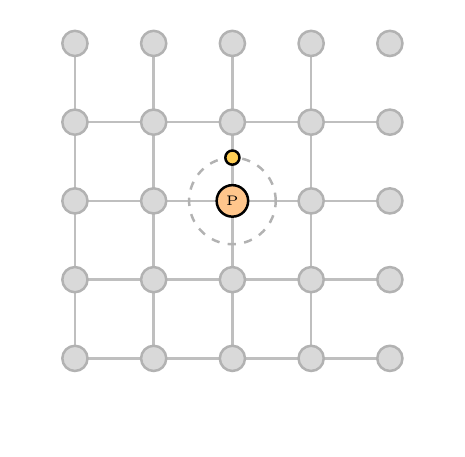
\begin{tikzpicture}[line width=0.9pt]
      \useasboundingbox (-0.6,-0.9) rectangle (4.6,4.2);

      % silicon lattice: grid of atoms with bonds
      \foreach \x in {0,1,2,3} {
        \foreach \y in {0,1,2,3} {
          \draw[gray!50] (\x,\y) -- (\x+1,\y);
          \draw[gray!50] (\x,\y) -- (\x,\y+1);
        }
      }
      \foreach \x in {0,...,4} {
        \foreach \y in {0,...,4} {
          \fill[gray!30] (\x,\y) circle (0.16);
          \draw[gray!60] (\x,\y) circle (0.16);
        }
      }

      % dopant atom (phosphorus) at center, replacing a silicon atom
      \fill[orange!45] (2,2) circle (0.2);
      \draw[black] (2,2) circle (0.2);
      \node[font=\tiny] at (2,2) {P};

      % spare electron near the dopant, loosely bound (dashed orbit)
      \draw[gray!60, dashed] (2,2) circle (0.55);
      \fill[myyellow] (2,2.55) circle (0.09);
      \draw (2,2.55) circle (0.09);

    \end{tikzpicture} \\[-3mm]
    \graytext{phosphorus donates a spare electron}\\
    \graytext{extra electrons are free to carry ($-$) charge}
  \end{minipage}%
  \begin{minipage}{0.5\textwidth}
    \centering
    \highlight{\textbf{p-type}} \\[3mm]
    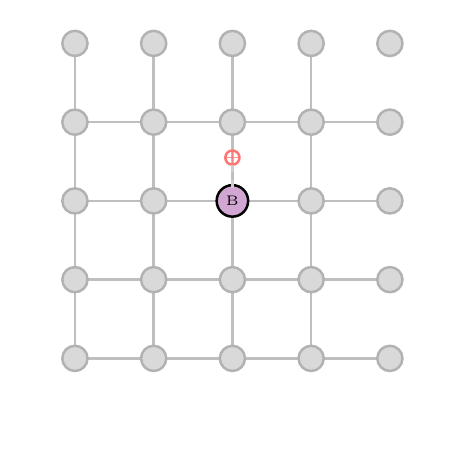
\begin{tikzpicture}[line width=0.9pt]
      \useasboundingbox (-0.6,-0.9) rectangle (4.6,4.2);

      % silicon lattice: grid of atoms with bonds
      \foreach \x in {0,1,2,3} {
        \foreach \y in {0,1,2,3} {
          \draw[gray!50] (\x,\y) -- (\x+1,\y);
          \draw[gray!50] (\x,\y) -- (\x,\y+1);
        }
      }
      \foreach \x in {0,...,4} {
        \foreach \y in {0,...,4} {
          \fill[gray!30] (\x,\y) circle (0.16);
          \draw[gray!60] (\x,\y) circle (0.16);
        }
      }

      % dopant atom (boron) at center, replacing a silicon atom
      \fill[violet!35] (2,2) circle (0.2);
      \draw[black] (2,2) circle (0.2);
      \node[font=\tiny] at (2,2) {B};

      % missing bond / hole next to the dopant
      \draw[red!55] (2,2.55) circle (0.09);
      \node[red!55, font=\tiny] at (2,2.55) {+};
      \draw[gray!40, dashed] (2,2.16) -- (2,2.46);

      \node[smallgraytext] at (2,-0.4) {};
    \end{tikzpicture} \\[-3mm]
    \graytext{boron leaves a missing bond (a hole)}\\
    \graytext{extra holes are free to carry ($+$) charge}
  \end{minipage}
  \\\vspace{2mm}
Adding a small amount of another element (called \highlight{\textbf{doping}}), creates extra electrons or extra holes (lack of electrons).
\end{frame}

\begin{frame}
  The source and the drain are made of one type and the base is made of another. The gate is separated from the base by an insulating layer.\\[3mm]
  \begin{minipage}{0.5\textwidth}
    \centering
    \highlight{\textbf{gate off} ($V_G = 0$)} \\[3mm]
    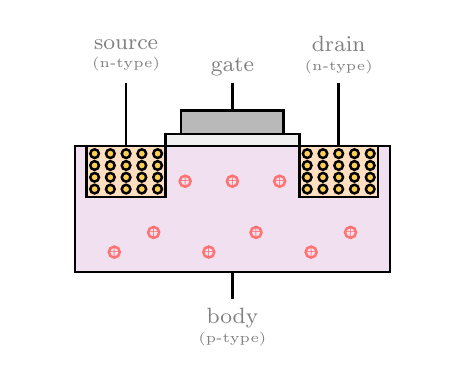
\begin{tikzpicture}[line width=0.9pt]
      \useasboundingbox (-0.6,-1.0) rectangle (4.6,3.1);

      % p-type substrate/body
      \filldraw[violet!12, draw=black] (0,0) rectangle (4,1.6);

      % n+ source and drain regions (copper colored)
      \filldraw[orange!25, draw=black] (0.15,0.95) rectangle (1.15,1.6);
      \filldraw[orange!25, draw=black] (2.85,0.95) rectangle (3.85,1.6);

      % gate oxide (insulator)
      \filldraw[gray!12, draw=black] (1.15,1.6) rectangle (2.85,1.75);
      % gate electrode
      \filldraw[gray!55, draw=black] (1.35,1.75) rectangle (2.65,2.05);

      % holes scattered in p-type body (sparse)
      \foreach \p in {(0.5,0.25),(1.0,0.5),(1.7,0.25),(2.0,1.15),
                      (2.3,0.5),(3.0,0.25),(3.5,0.5),(1.4,1.15),(2.6,1.15)} {
        \draw[red!55] \p circle (0.07);
        \node[red!55, font=\tiny] at \p {+};
      }

      % electrons evenly packed in source
      \foreach \x in {0.25,0.45,0.65,0.85,1.05} {
        \foreach \y in {1.05,1.2,1.35,1.5} {
          \fill[myyellow] (\x,\y) circle (0.055);
          \draw (\x,\y) circle (0.055);
        }
      }
      % electrons evenly packed in drain
      \foreach \x in {2.95,3.15,3.35,3.55,3.75} {
        \foreach \y in {1.05,1.2,1.35,1.5} {
          \fill[myyellow] (\x,\y) circle (0.055);
          \draw (\x,\y) circle (0.055);
        }
      }

      % contacts
      \draw (0.65,1.6) -- (0.65,2.4);
      \node[smallgraytext, align=center] at (0.65,2.75) {source\\[-1mm]{\tiny (n-type)}};
      \draw (3.35,1.6) -- (3.35,2.4);
      \node[smallgraytext, align=center] at (3.35,2.75) {drain\\[-1mm]{\tiny (n-type)}};
      \draw (2.0,2.05) -- (2.0,2.4);
      \node[smallgraytext] at (2.0,2.6) {gate};
      \draw (2.0,0) -- (2.0,-0.35);
      \node[smallgraytext, align=center] at (2.0,-0.7) {body\\[-1mm]{\tiny (p-type)}};
    \end{tikzpicture} \\[3mm]
    \graytext{few free electrons in the base}\\[-1mm]
    \graytext{disturbance cannot move across base}
  \end{minipage}%
  \begin{minipage}{0.5\textwidth}
    \centering
    \highlight{\textbf{gate on} ($V_G > V_{th}$)} \\[3mm]
    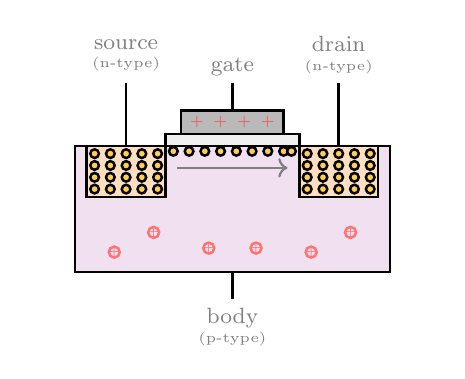
\begin{tikzpicture}[line width=0.9pt]
      \useasboundingbox (-0.6,-1.0) rectangle (4.6,3.1);

      % p-type substrate/body
      \filldraw[violet!12, draw=black] (0,0) rectangle (4,1.6);

      % n+ source and drain regions (copper colored)
      \filldraw[orange!25, draw=black] (0.15,0.95) rectangle (1.15,1.6);
      \filldraw[orange!25, draw=black] (2.85,0.95) rectangle (3.85,1.6);

      % gate oxide (insulator)
      \filldraw[gray!12, draw=black] (1.15,1.6) rectangle (2.85,1.75);
      % gate electrode, positively charged
      \filldraw[gray!55, draw=black] (1.35,1.75) rectangle (2.65,2.05);
      \foreach \gx in {1.55,1.85,2.15,2.45} {
        \node[red!70, font=\tiny] at (\gx,1.9) {+};
      }

      % holes scattered in p-type body, away from the surface
      \foreach \p in {(0.5,0.25),(1.0,0.5),(1.7,0.3),(2.3,0.3),(3.0,0.25),(3.5,0.5)} {
        \draw[red!55] \p circle (0.07);
        \node[red!55, font=\tiny] at \p {+};
      }

      % electrons evenly packed in source
      \foreach \x in {0.25,0.45,0.65,0.85,1.05} {
        \foreach \y in {1.05,1.2,1.35,1.5} {
          \fill[myyellow] (\x,\y) circle (0.055);
          \draw (\x,\y) circle (0.055);
        }
      }
      % electrons evenly packed in drain
      \foreach \x in {2.95,3.15,3.35,3.55,3.75} {
        \foreach \y in {1.05,1.2,1.35,1.5} {
          \fill[myyellow] (\x,\y) circle (0.055);
          \draw (\x,\y) circle (0.055);
        }
      }
      % thin row of electrons connecting source to drain
      \foreach \x in {1.25,1.45,1.65,1.85,2.05,2.25,2.45,2.65,2.75} {
        \fill[myyellow] (\x,1.53) circle (0.055);
        \draw (\x,1.53) circle (0.055);
      }
      % small arrows showing the channel electrons are drawn up from source/drain

      % flow arrow (reversed direction, source to drain)
      \draw[->, gray, thick] (1.3,1.32) -- (2.7,1.32);

      % contacts
      \draw (0.65,1.6) -- (0.65,2.4);
      \node[smallgraytext, align=center] at (0.65,2.75) {source\\[-1mm]{\tiny (n-type)}};
      \draw (3.35,1.6) -- (3.35,2.4);
      \node[smallgraytext, align=center] at (3.35,2.75) {drain\\[-1mm]{\tiny (n-type)}};
      \draw (2.0,2.05) -- (2.0,2.4);
      \node[smallgraytext] at (2.0,2.6) {gate};
      \draw (2.0,0) -- (2.0,-0.35);
      \node[smallgraytext, align=center] at (2.0,-0.7) {body\\[-1mm]{\tiny (p-type)}};
    \end{tikzpicture} \\[3mm]
    \graytext{electrons drawn from source and drain}\\[-1mm]
    \graytext{disturbance can move across base}
  \end{minipage}
  \\[4mm]
  The gate voltage controls whether electrons connect the source and drain.
\end{frame}

\begin{frame}
\begin{center}
    \highlight{\large \texttt{NOT}\;\textbf{gate}}
\end{center}
  \begin{minipage}{0.45\textwidth}
    \centering
    \begin{tikzpicture}
      \node[smallgraytext] at (0,2.15) {high};
      \draw[thick] (-0.4,1.9) -- (0.4,1.9);
      \draw[thick] (0,1.9) -- (0,1.6);
      \pic at (0,1.0) {pmos};
      \pic at (0,-1.0) {nmos};
      \draw[thick] (0,0.4) -- (0,-0.4);
      \fill (0,0) circle (1.4pt);
      \draw[thick] (0,0) -- (1.1,0) node[right, smallgraytext] {\ttab{y}};
      \draw[thick] (0,-1.6) -- (0,-1.9);
      \draw[thick] (-0.4,-1.9) -- (0.4,-1.9);
      \node[smallgraytext] at (0,-2.15) {low};
      % pushed the gate lead out further so the label clears the pic
      \draw[thick] (-0.6,1.0) -| (-1.3,0) |- (-0.6,-1.0);
      \draw[thick] (-1.3,0) -- ++(-0.5,0) node[left, smallgraytext] {\ttab{a}};
      \fill (-1.3,0) circle (1.4pt);
    \end{tikzpicture}
  \end{minipage}%
  \begin{minipage}{0.5\textwidth}
    \centering
    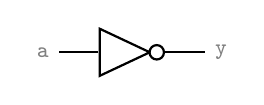
\begin{tikzpicture}
      \node[not gate US, draw, thick, scale=1.3] (n) at (0,0) {};
      \draw[thick] (n.input) -- ++(-0.5,0) node[left, smallgraytext] {\ttab{a}};
      \draw[thick] (n.output) -- ++(0.5,0) node[right, smallgraytext] {\ttab{y}};
    \end{tikzpicture} \\[6mm]
    \renewcommand{\arraystretch}{1.3}
    \begin{tabular}{c|c}
      \ttab{a} & \ttab{y} \\ \hline
      \ttab{0} & \ttab{1} \\
      \ttab{1} & \ttab{0} \\
    \end{tabular}
  \end{minipage}
  \begin{center}
          \graytext{the transistor circuit, circuit symbol, and truth table for the \texttt{NOT} gate}
  \end{center}
\end{frame}

\begin{frame}
\begin{center}
    \highlight{\large \texttt{AND}\;\textbf{gate}}
\end{center}
  \begin{minipage}{0.45\textwidth}
    \centering
    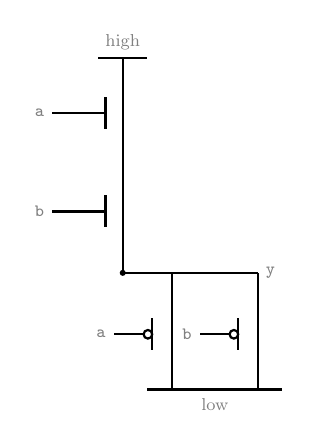
\begin{tikzpicture}[scale=0.78, every node/.style={transform shape}]
      \node[smallgraytext] at (0,2.75) {high};
      \draw[thick] (-0.4,2.5) -- (0.4,2.5);
      \draw[thick] (0,2.5) -- (0,2.2);
      \pic at (0,1.6) {nmos};
      % longer lead so label clears the pic and the vertical bus below
      \draw[thick] (-0.6,1.6) -- ++(-0.55,0) node[left, smallgraytext] {\ttab{a}};
      \draw[thick] (0,1.0) -- (0,0.6);
      \pic at (0,0.0) {nmos};
      \draw[thick] (-0.6,0.0) -- ++(-0.55,0) node[left, smallgraytext] {\ttab{b}};
      \draw[thick] (0,-0.6) -- (0,-1.0);
      \fill (0,-1.0) circle (1.4pt);
      \draw[thick] (0,-1.0) -- (2.2,-1.0) node[right, smallgraytext] {\ttab{y}};
      % nudged the two pMOS further apart so their gate leads don't
      % run into each other's transistor symbol
      \pic at (0.8,-2.0) {pmos};
      \pic at (2.2,-2.0) {pmos};
      \draw[thick] (0.8,-1.4) -- (0.8,-1.0);
      \draw[thick] (2.2,-1.4) -- (2.2,-1.0);
      \draw[thick] (0.8,-2.6) -- (0.8,-2.9);
      \draw[thick] (2.2,-2.6) -- (2.2,-2.9);
      \draw[thick] (0.4,-2.9) -- (2.6,-2.9);
      \node[smallgraytext] at (1.5,-3.15) {low};
      \draw[thick] (0.2,-2.0) -- ++(-0.35,0) node[left, smallgraytext] {\ttab{a}};
      \draw[thick] (1.6,-2.0) -- ++(-0.35,0) node[left, smallgraytext] {\ttab{b}};
    \end{tikzpicture}
  \end{minipage}%
  \begin{minipage}{0.5\textwidth}
    \centering
    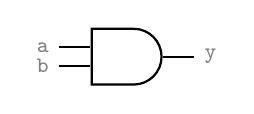
\begin{tikzpicture}
      \node[and gate US, draw, thick, scale=1.2] (g) at (0,0) {};
      \draw[thick] (g.input 1) -- ++(-0.4,0) node[left, smallgraytext] {\ttab{a}};
      \draw[thick] (g.input 2) -- ++(-0.4,0) node[left, smallgraytext] {\ttab{b}};
      \draw[thick] (g.output) -- ++(0.4,0) node[right, smallgraytext] {\ttab{y}};
    \end{tikzpicture} \\[6mm]
    \renewcommand{\arraystretch}{1.2}
    \begin{tabular}{cc|c}
      \ttab{a} & \ttab{b} & \ttab{y} \\ \hline
      \ttab{0} & \ttab{0} & \ttab{0} \\
      \ttab{0} & \ttab{1} & \ttab{0} \\
      \ttab{1} & \ttab{0} & \ttab{0} \\
      \ttab{1} & \ttab{1} & \ttab{1} \\
    \end{tabular}
  \end{minipage}
  \begin{center}
    \graytext{the transistor circuit, circuit symbol, and truth table for the \texttt{AND} gate}
  \end{center}
\end{frame}

\begin{frame}
\begin{center}
    \highlight{\large \texttt{OR}\;\textbf{gate}}
\end{center}
  \begin{minipage}{0.45\textwidth}
    \centering
    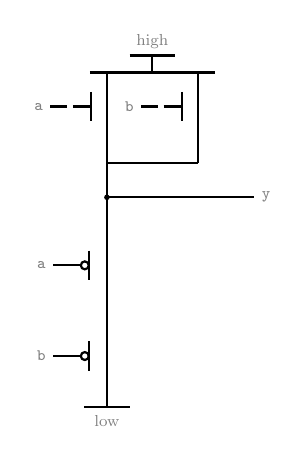
\begin{tikzpicture}[scale=0.72, every node/.style={transform shape}]
      \node[smallgraytext] at (1.5,2.75) {high};
      \draw[thick] (1.1,2.5) -- (1.9,2.5);
      \draw[thick] (1.5,2.5) -- (1.5,2.2);
      \draw[thick] (0.4,2.2) -- (2.6,2.2);
      % pushed the parallel nMOS further apart so the "b" lead
      % no longer cuts through the "a" transistor's symbol
      \pic at (0.7,1.6) {nmos};
      \pic at (2.3,1.6) {nmos};
      \draw[thick] (0.0,1.6) -- ++(-0.3,0) node[left, smallgraytext] {\ttab{a}};
      \draw[thick] (1.6,1.6) -- ++(-0.3,0) node[left, smallgraytext] {\ttab{b}};
      \draw[thick] (0.7,1.0) -- (0.7,0.6);
      \draw[thick] (2.3,1.0) -- (2.3,0.6);
      \draw[thick] (0.7,0.6) -- (2.3,0.6);
      \draw[thick] (0.7,0.6) -- (0.7,0.0);
      \fill (0.7,0.0) circle (1.4pt);
      \draw[thick] (0.7,0.0) -- (3.3,0.0) node[right, smallgraytext] {\ttab{y}};
      \draw[thick] (0.7,0.0) -- (0.7,-0.6);
      \pic at (0.7,-1.2) {pmos};
      \draw[thick] (0.1,-1.2) -- ++(-0.35,0) node[left, smallgraytext] {\ttab{a}};
      \draw[thick] (0.7,-1.8) -- (0.7,-2.2);
      \pic at (0.7,-2.8) {pmos};
      \draw[thick] (0.1,-2.8) -- ++(-0.35,0) node[left, smallgraytext] {\ttab{b}};
      \draw[thick] (0.7,-3.4) -- (0.7,-3.7);
      \draw[thick] (0.3,-3.7) -- (1.1,-3.7);
      \node[smallgraytext] at (0.7,-3.95) {low};
    \end{tikzpicture}
  \end{minipage}%
  \begin{minipage}{0.5\textwidth}
    \centering
    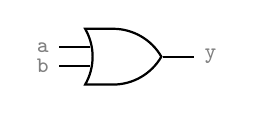
\begin{tikzpicture}
      \node[or gate US, draw, thick, scale=1.2] (g) at (0,0) {};
      \draw[thick] (g.input 1) -- ++(-0.4,0) node[left, smallgraytext] {\ttab{a}};
      \draw[thick] (g.input 2) -- ++(-0.4,0) node[left, smallgraytext] {\ttab{b}};
      \draw[thick] (g.output) -- ++(0.4,0) node[right, smallgraytext] {\ttab{y}};
    \end{tikzpicture} \\[6mm]
    \renewcommand{\arraystretch}{1.2}
    \begin{tabular}{cc|c}
      \ttab{a} & \ttab{b} & \ttab{y} \\ \hline
      \ttab{0} & \ttab{0} & \ttab{0} \\
      \ttab{0} & \ttab{1} & \ttab{1} \\
      \ttab{1} & \ttab{0} & \ttab{1} \\
      \ttab{1} & \ttab{1} & \ttab{1} \\
    \end{tabular}
  \end{minipage}
  \begin{center}
    \graytext{the transistor circuit, circuit symbol, and truth table for the \texttt{OR} gate}
  \end{center}
\end{frame}


\begin{frame}
  Adding a \texttt{NOT} gate to the output of an \texttt{AND} gate or \texttt{OR} gate gives two more gates (a \texttt{NAND} and a \texttt{NOR}, respectively), drawn with a circle on the output.\\[4mm]
  \begin{minipage}{0.5\textwidth}
    \centering
    \highlight{\texttt{NAND}\;\textbf{gate}} \\[3mm]
    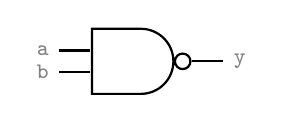
\begin{tikzpicture}
      \node[nand gate US, draw, thick, scale=1.4] (g) at (0,0) {};
      \draw[thick] (g.input 1) -- ++(-0.4,0) node[left, smallgraytext] {\ttab{a}};
      \draw[thick] (g.input 2) -- ++(-0.4,0) node[left, smallgraytext] {\ttab{b}};
      \draw[thick] (g.output) -- ++(0.4,0) node[right, smallgraytext] {\ttab{y}};
    \end{tikzpicture} \\[3mm]
    \graytext{\ttab{1} unless both inputs are \ttab{1}} \\[4mm]
    \renewcommand{\arraystretch}{1.2}
    \begin{tabular}{cc|c}
      \ttab{a} & \ttab{b} & \ttab{y} \\ \hline
      \ttab{0} & \ttab{0} & \ttab{1} \\
      \ttab{0} & \ttab{1} & \ttab{1} \\
      \ttab{1} & \ttab{0} & \ttab{1} \\
      \ttab{1} & \ttab{1} & \ttab{0} \\
    \end{tabular}
  \end{minipage}%
  \begin{minipage}{0.5\textwidth}
    \centering
    \highlight{\texttt{NOR}\;\textbf{gate}} \\[3mm]
    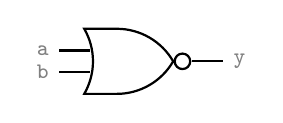
\begin{tikzpicture}
      \node[nor gate US, draw, thick, scale=1.4] (g) at (0,0) {};
      \draw[thick] (g.input 1) -- ++(-0.4,0) node[left, smallgraytext] {\ttab{a}};
      \draw[thick] (g.input 2) -- ++(-0.4,0) node[left, smallgraytext] {\ttab{b}};
      \draw[thick] (g.output) -- ++(0.4,0) node[right, smallgraytext] {\ttab{y}};
    \end{tikzpicture} \\[3mm]
    \graytext{\ttab{1} only when both inputs are \ttab{0}} \\[4mm]
    \renewcommand{\arraystretch}{1.2}
    \begin{tabular}{cc|c}
      \ttab{a} & \ttab{b} & \ttab{y} \\ \hline
      \ttab{0} & \ttab{0} & \ttab{1} \\
      \ttab{0} & \ttab{1} & \ttab{0} \\
      \ttab{1} & \ttab{0} & \ttab{0} \\
      \ttab{1} & \ttab{1} & \ttab{0} \\
    \end{tabular}
  \end{minipage}
\end{frame}

\begin{frame}
\begin{center}
    \highlight{\large \texttt{XOR}\;\textbf{gate}}
\end{center}
  We can build an exclusive \texttt{OR} gate (\texttt{XOR} gate) by combining an \texttt{OR} gate and a \texttt{NAND} gate.\\[4mm]
  \begin{center}
  \begin{minipage}{0.5\textwidth}
    \centering
    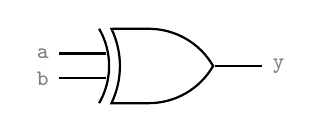
\begin{tikzpicture}
      \node[xor gate US, draw, thick, scale=1.6] (g) at (0,0) {};
      \draw[thick] (g.input 1) -- ++(-0.6,0) node[left, smallgraytext] {\ttab{a}};
      \draw[thick] (g.input 2) -- ++(-0.6,0) node[left, smallgraytext] {\ttab{b}};
      \draw[thick] (g.output) -- ++(0.6,0) node[right, smallgraytext] {\ttab{y}};
    \end{tikzpicture} \\[6mm]
    \renewcommand{\arraystretch}{1.2}
    \begin{tabular}{cc|c}
      \ttab{a} & \ttab{b} & \ttab{y} \\ \hline
      \ttab{0} & \ttab{0} & \ttab{0} \\
      \ttab{0} & \ttab{1} & \ttab{1} \\
      \ttab{1} & \ttab{0} & \ttab{1} \\
      \ttab{1} & \ttab{1} & \ttab{0} \\
    \end{tabular}
  \end{minipage}
  \end{center}
  \begin{center}
    \graytext{output is \ttab{1} when the inputs differ}
  \end{center}
\end{frame}

\begin{frame}
  \begin{center}
    These few gates are enough to build every circuit in the rest of the course.
  \end{center}
\end{frame}

\end{document}
